\documentclass[a4paper]{article}
\addtolength{\hoffset}{-2.25cm}
\addtolength{\textwidth}{4.5cm}
\addtolength{\voffset}{-3.25cm}
\addtolength{\textheight}{5cm}
\setlength{\parskip}{0pt}
\setlength{\parindent}{0in}

\usepackage[square,sort,comma,numbers]{natbib}
\usepackage{blindtext} % Package to generate dummy text
\usepackage{charter} % Use the Charter font
\usepackage[utf8]{inputenc} % Use UTF-8 encoding
\usepackage{microtype} % Slightly tweak font spacing for aesthetics
\usepackage{amsthm, amsmath, amssymb} % Mathematical typesetting
\usepackage{float} % Improved interface for floating objects
\usepackage{hyperref} % For hyperlinks in the PDF
\usepackage{graphicx, multicol} % Enhanced support for graphics
\usepackage{xcolor} % Driver-independent color extensions
\usepackage{pseudocode} % Environment for specifying algorithms in a natural way
\usepackage[mmddyy]{datetime} % Uses YEAR-MONTH-DAY format for dates

\usepackage{fancyhdr} % Headers and footers
\pagestyle{fancy} % All pages have headers and footers
\fancyhead{}\renewcommand{\headrulewidth}{0pt} % Blank out the default header
\fancyfoot[L]{} % Custom footer text
\fancyfoot[C]{} % Custom footer text
\fancyfoot[R]{\thepage} % Custom footer text
\newcommand{\note}[1]{\marginpar{\scriptsize \textcolor{red}{#1}}} % Enables comments in red on margin

\DeclareMathOperator*{\argmin}{arg\,min}

%----------------------------------------------------------------------------------------

\newcommand{\yourname}{Balthazar Neveu}
\newcommand{\youremail}{balthazarneveu@gmail.com}
\newcommand{\assignmentnumber}{7}

\begin{document}

\fancyhead[C]{}
\hrule \medskip
\begin{minipage}{0.295\textwidth} 
\raggedright
\footnotesize
\yourname \hfill\\
\youremail
\end{minipage}
\begin{minipage}{0.4\textwidth} 
\centering 
\large 
Lab session \# \assignmentnumber\\ 
\normalsize 
ALTEGRAD 2023\\ 
\end{minipage}
\begin{minipage}{0.295\textwidth} 
\raggedleft
\today\hfill\\
\end{minipage}
\medskip\hrule 
\bigskip


\section*{Code}

More info:
\href{https://github.com/balthazarneveu/MVA23_ALTEGRAD/#readme}{MVA ALTEGRAD Balthazar Neveu on Github}

\section*{DeepSets: Learn to add \textit{(add to learn...)}}
\section*{Question 1 : LSTM are not permutation invariant, therefore not recommended for sets processing}
Permutation invariance refers to the property where the model's output does not change if the order of the input data is changed. For instance, in a permutation invariant model, the input sequence [1, 2, 3] would yield the same output as [3, 2, 1]. Permuation invaraiance is a desirable property to deal with sets.
\newline
Long Short-Term Memory (LSTM) models are not permutation invariant. LSTM process sequential data in a recurrent fashion and maintain a kind of memory. Order matters for natural language processing or time series but not for sets. 

LSTM are therefore not suited for sets processing.
\newline



We confirm this with the figure \ref{fig:performances_deepset_lstm_evolution} from task 7.

\begin{figure}[h]
    \centering
    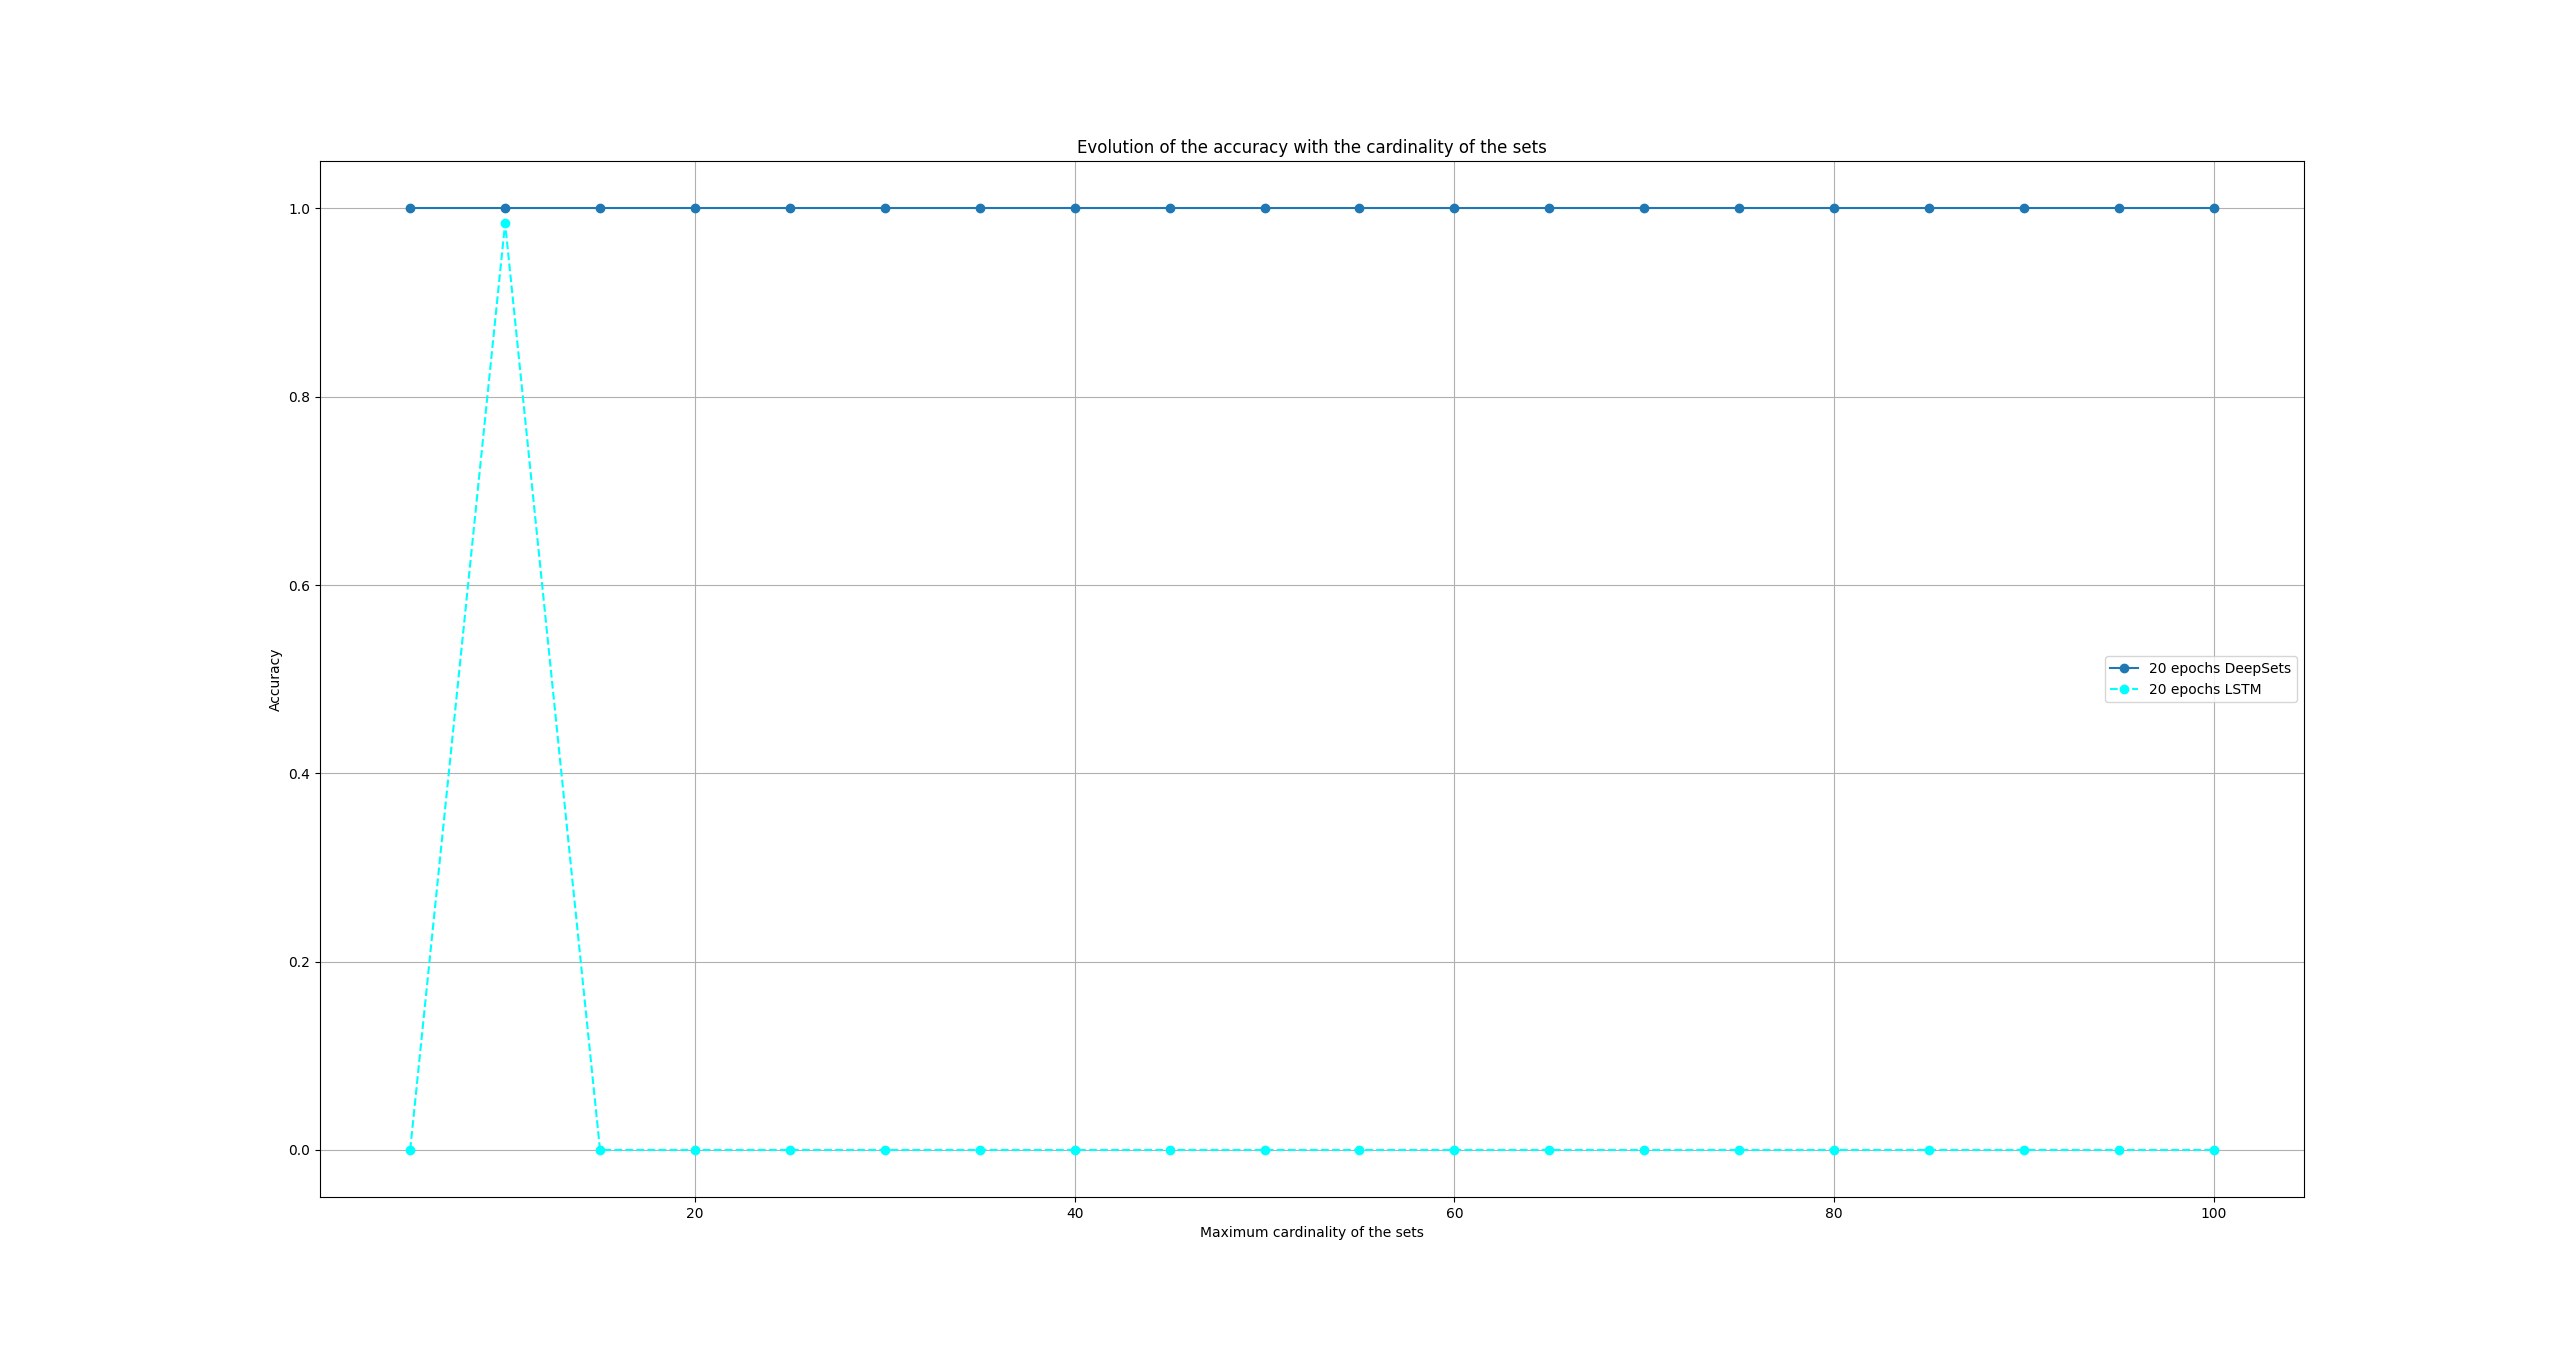
\includegraphics[width=1.\textwidth]{figures/deep_set_performances.png}
    \caption{Comparison of accuracies of the prediction of the sum over a set of integers with regard to the cardinality of the set. Deepset is able to generalize while LSTM fails (only rougly correct when summing 10 digits, in the regime it was trained).}
    \label{fig:performances_deepset_lstm}
\end{figure}

\subsection*{Task 7}
Please note that this figure may be a bit misleading  as the results of deepSet look almost too good to be true (100\% accuracy), which is why I also report the accuracies of Deepset and LSTM while training \ref{fig:performances_deepset_lstm_evolution}.
Rounding the predictions while estimating the accuracy (as a classification) also lets us think that the DeepSet model perfectly learnt how to add integers. This is not totally true if we take a careful look at the Mean Absolute Error (MAE) which is around 0.2 when we sum 100 integers. \ref{fig:mean_absolute_error_deepset_lstm_evolution}.

\subsubsection*{100\% accuracy = learn to add ... add to learn - Interpretation (out-of-scope)}
\textit{It is important to note that one can think of learning the addition on a set as a degenerate case for the Deepset architecture.}
\newline
Special embeddings like $[1, 1, 1, 1, 0, ..., 0]$ can encode the digit $4=1+1+1+1$...  since a fully connected layer can simply perform identity mapping, the pooling sum across the set can  perform the actual sums on each component of the hidden vectors... which is the actual task we're learning here. The availabiltiy of the sum operation in the pooling layer is the key to this trick. The final fully connected layer can compensate the $tanh$ non linearity ($tanh(1)\approx{0.76}$, $tanh(0)=0$). There may be many other ways to achieve this, but this one is the simplest I can think of.
\newline
\textbf{Multiplication would probably be much harder.}


\begin{figure}[h]
    \centering
    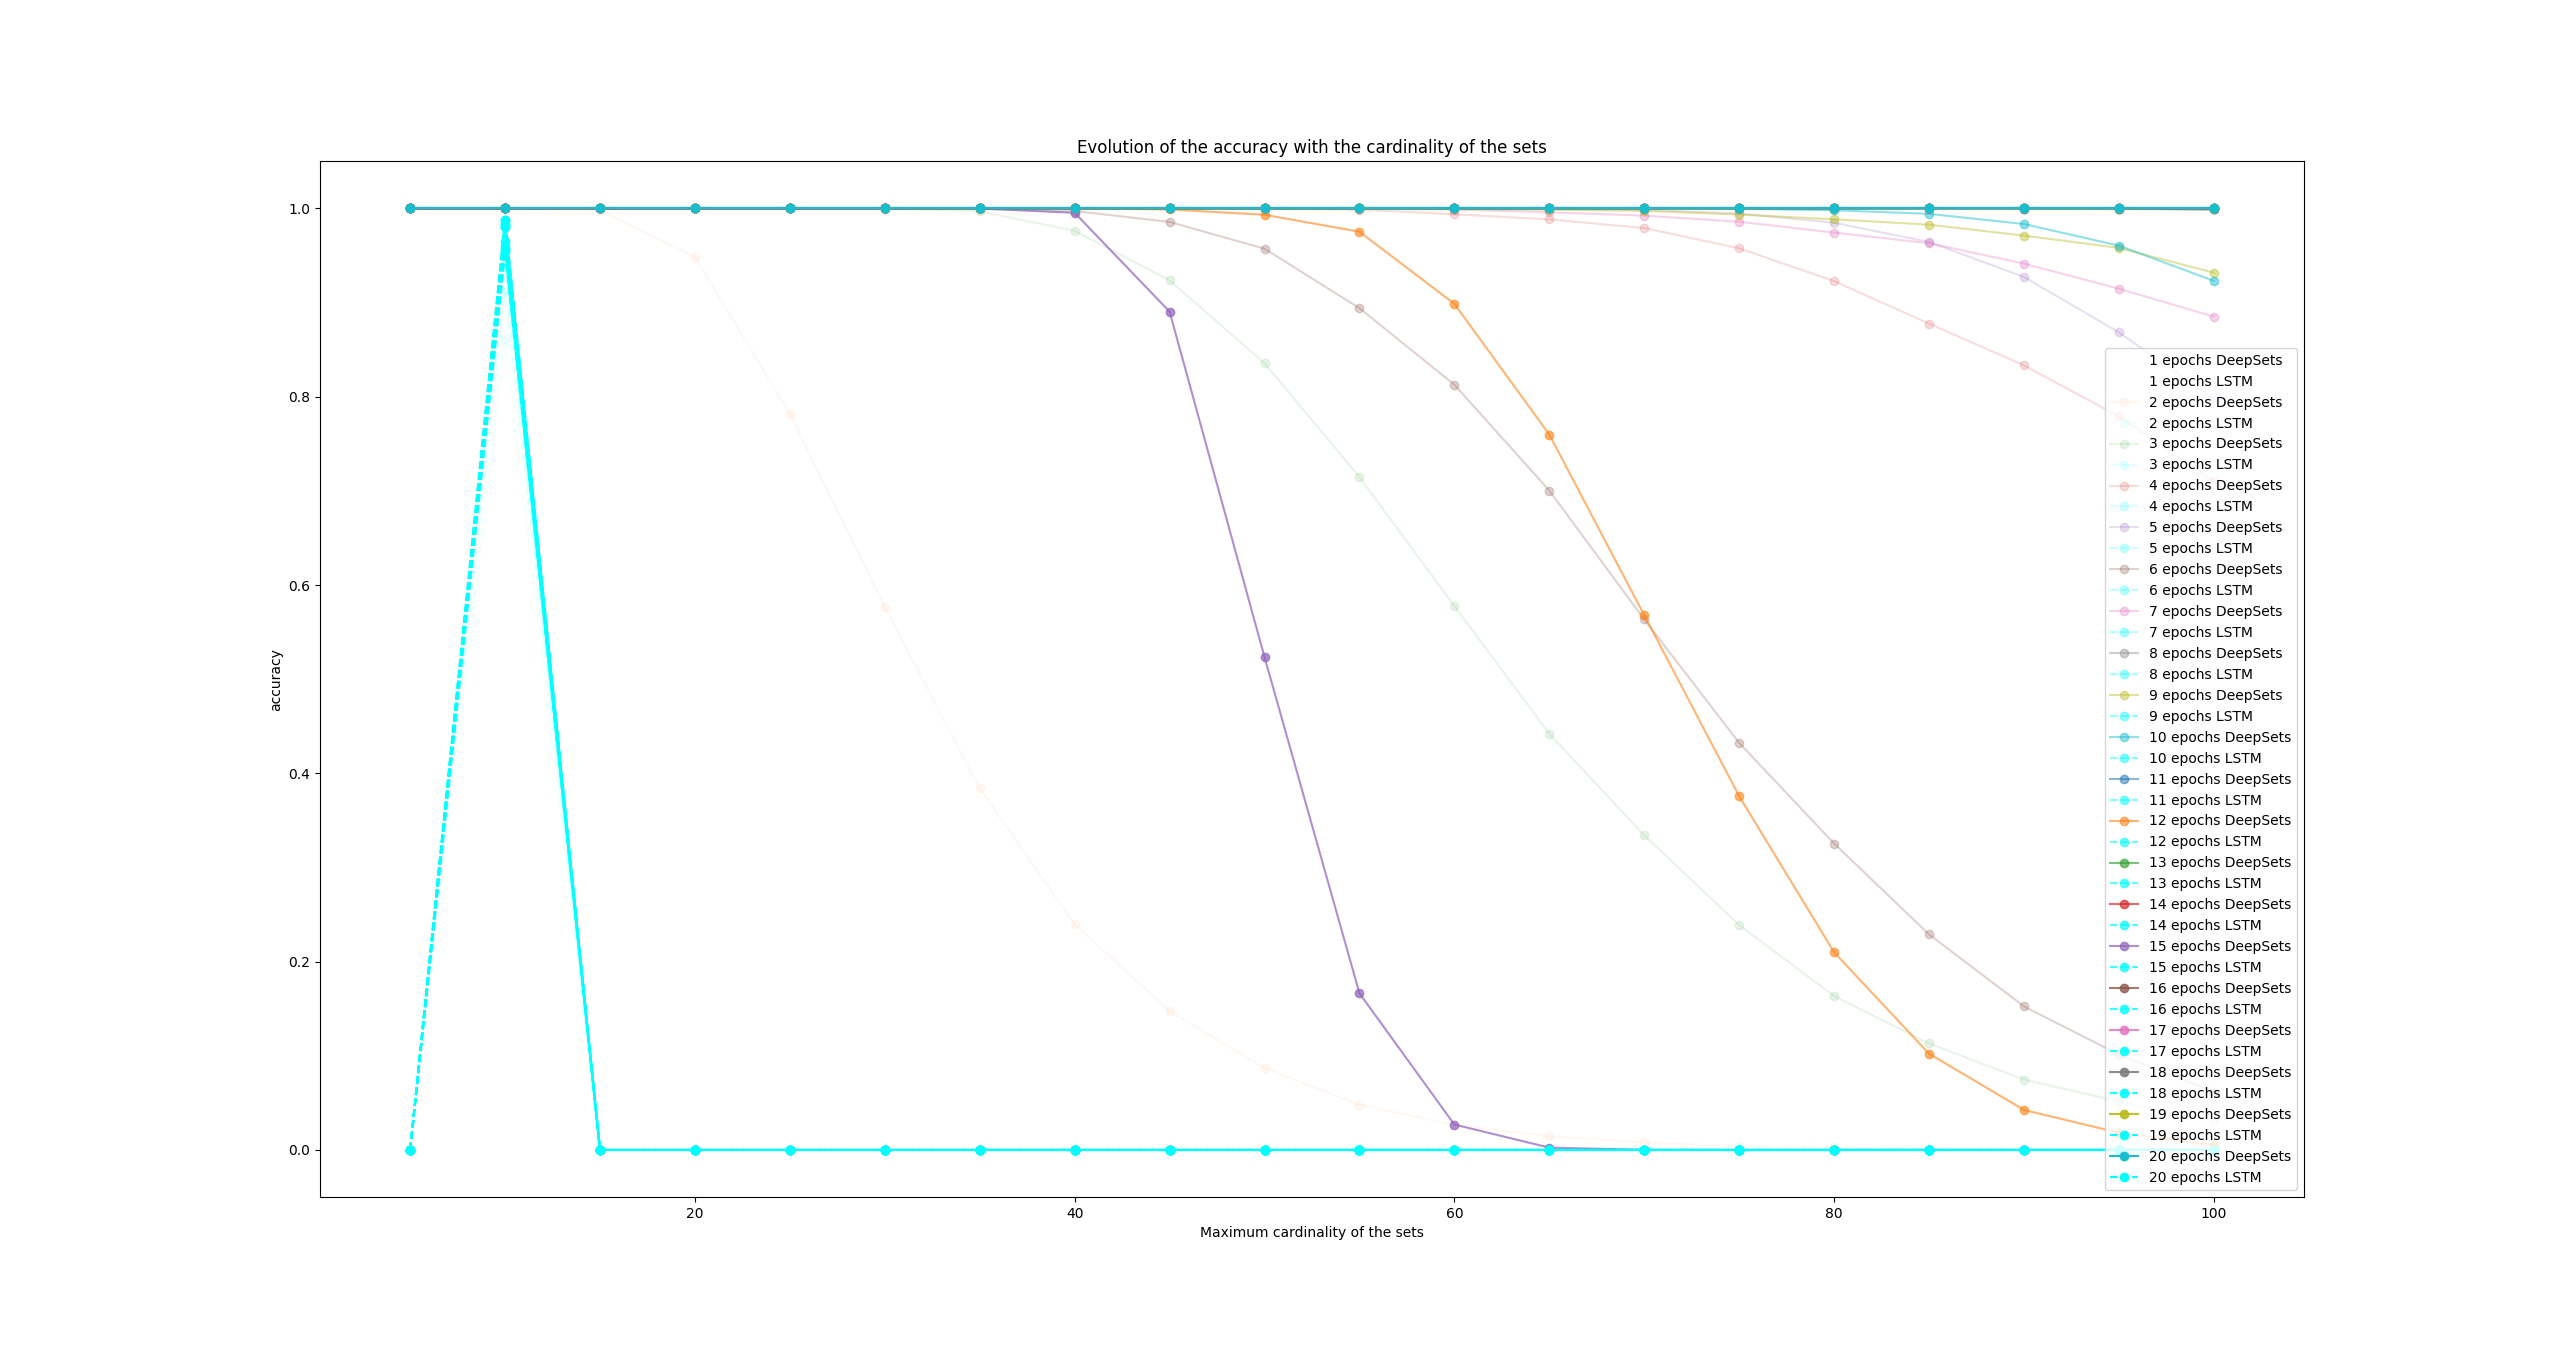
\includegraphics[width=1.\textwidth]{figures/deep_set_performances_evol.png}
    \caption{Evolution of the accuracies regarding cardinality during training}
    \label{fig:performances_deepset_lstm_evolution}
\end{figure}

\begin{figure}[h]
    \centering
    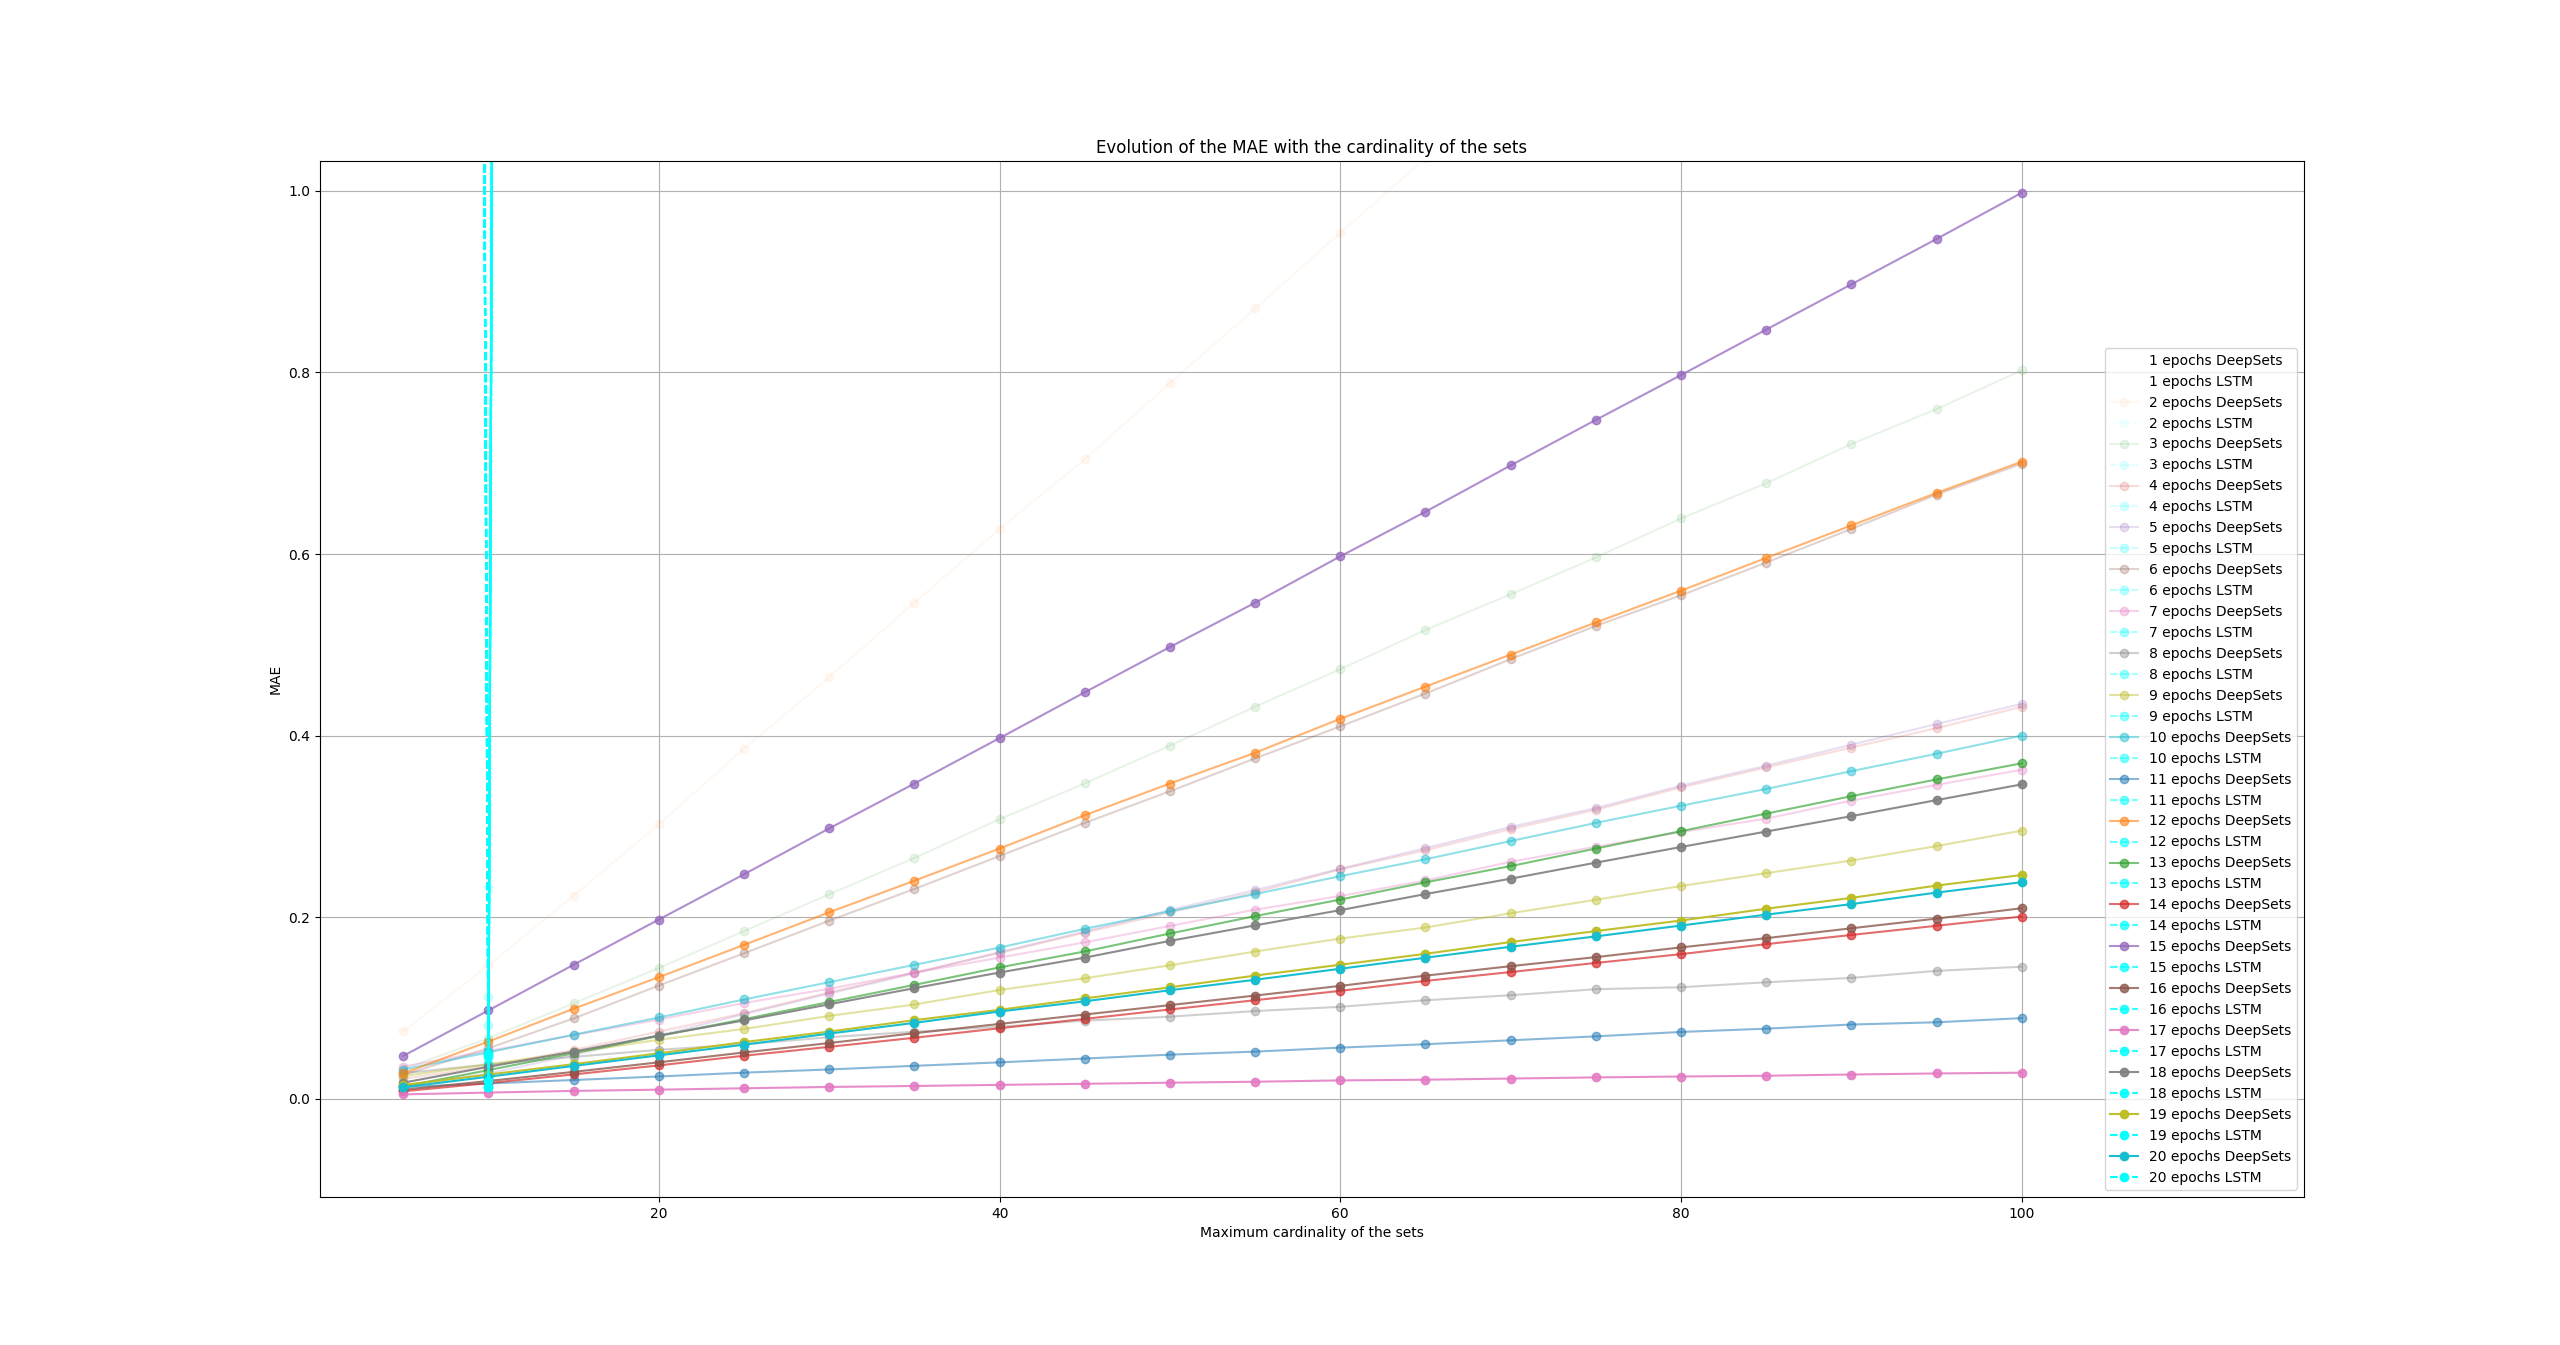
\includegraphics[width=1.\textwidth]{figures/deep_set_performances_MAE_evol.png}
    \caption{Evolution of Mean Absolute error regarding cardinality, during training}
    \label{fig:mean_absolute_error_deepset_lstm_evolution}
\end{figure}


\section*{Question 2 : GNN vs DeepSet}
Graph Neural Networks for graph-level tasks use graph structures to detect patterns (like graph classification) or properties. Deepsets do not consider edges between nodes except self loops.
\textbf{GNN use aggregation/message passing layers to propagate information between nodes. Deepset does not.}
\newline
\textbf{What GNN for graph-level tasks and DeepSet have in common is the readout function (a.k.a. pooling layer).}

Although there's no explicit ordering between the nodes, the relationship between nodes is considered in the GNN architecture: aggregation layers relies on the permutation equivariance.

We can consider of DeepSet as a degenerate instance of GNN. 2 options to understand the concept.
\begin{itemize}
    \item Deepset is an instance of GNN where the aggregation layers are discarded. The fully connected layers, non linear activations and readout function (global pooling) are the layers in common.
    \item Deepset is an instance of GNN where the agrregation layers are used but with a degenerate graph construction where nodes are isolated (degree 0, no edges except self loops). The adjacency matrix becomes the identity matrix.
\end{itemize}
Processing a set using DeepSet or a GNN with a degenerate edgeless graph construction with only self loops is mathematically equivalent.

Finally, DeepSet is a permutation invariant architecture. It is not suited for graph-level tasks where structure matters.


\section*{Question 3 : }

\section*{Question 4 : Generate non binary graphs - use the Frobenius norm}
Instead of using the binary cross entropy loss, we can use the \textbf{mean squared error} loss on all elements of the error matrix $A-\tilde{A}$ if we want to generalize to non binary edges graphs generations.
$$\text{MSE} = \frac{1}{n^2} \sum_{i=1}^n \sum_{j=1}^n (\tilde{A}_{ij} - A_{ij})^2$$
\textit{The binary cross entropy loss is a good choice for classification problems}, but is not suited for regression problems.

% The binary cross-entropy loss function, as described in your question, is indeed well-suited for unweighted graphs where the adjacency matrix consists of binary values (0 or 1). However, for weighted graphs, where the adjacency matrix contains a range of values (not limited to just 0 or 1), a different loss function would be more appropriate.

% One such loss function that could be used for weighted graphs is the Mean Squared Error (MSE) loss. The MSE loss measures the average of the squares of the errors—that is, the average squared difference between the estimated values and the actual value. This is suitable for weighted graphs as it can effectively capture the variance between the predicted weighted edges and the actual weights in the graph.

% The MSE loss for a weighted graph can be formulated as follows:

% \[ \text{MSE} = \frac{1}{n^2} \sum_{i=1}^n \sum_{j=1}^n (\tilde{A}_{ij} - A_{ij})^2 \]

% Here, \( \tilde{A}_{ij} \) represents the predicted weight between nodes \( i \) and \( j \) in the reconstructed adjacency matrix, and \( A_{ij} \) is the actual weight in the original adjacency matrix. The summation is done over all pairs of nodes, and the result is normalized by the total number of pairs \( n^2 \).

% This loss function is more appropriate for weighted graphs as it takes into account the actual numerical values in the adjacency matrix and penalizes deviations from these values, whether they are greater or less than the predicted values. It's especially suitable for scenarios where the weights represent important quantitative measures, like the strength of the connection between nodes in the graph.



% \bibliographystyle{plain}
% \bibliography{references}



\begin{figure}[ht!]
    \centering
    % Graph 00
    \begin{minipage}{.45\textwidth}
      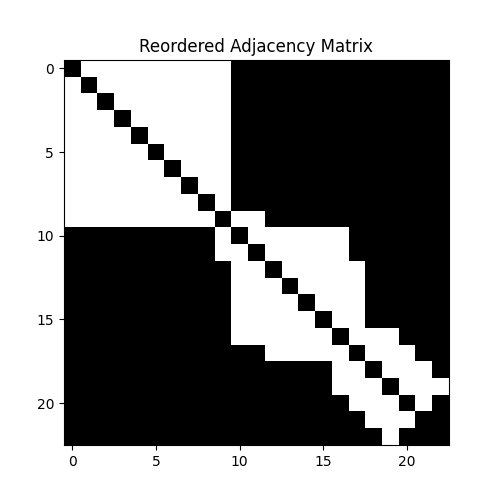
\includegraphics[width=0.7\linewidth]{figures/graph_00_adjacency_matrix.png}
    \end{minipage}\hfill
    \begin{minipage}{.45\textwidth}
      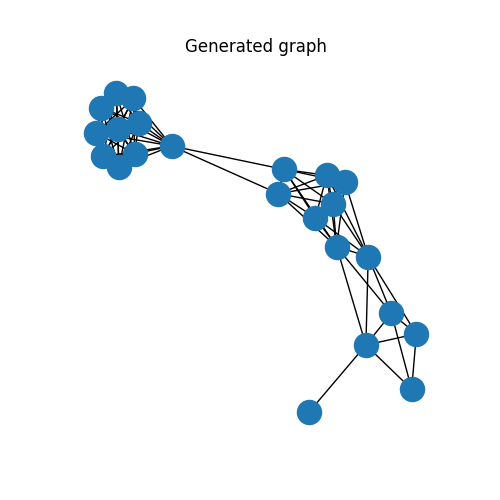
\includegraphics[width=0.7\linewidth]{figures/graph_00_generated_graph.png}
    \end{minipage}
  
    % Graph 01
    \begin{minipage}{.45\textwidth}
      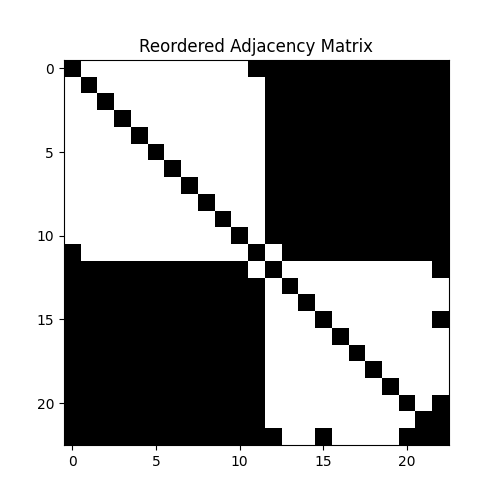
\includegraphics[width=0.7\linewidth]{figures/graph_01_adjacency_matrix.png}
    \end{minipage}\hfill
    \begin{minipage}{.45\textwidth}
      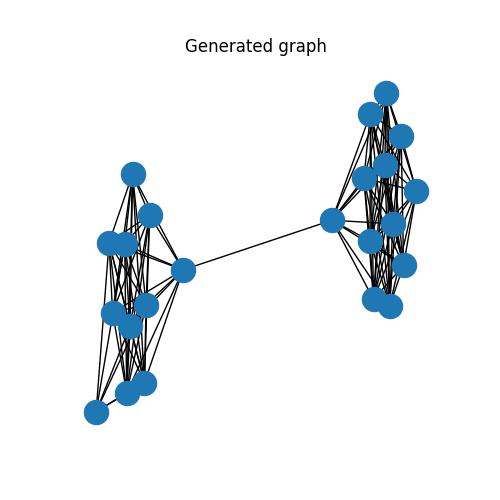
\includegraphics[width=0.7\linewidth]{figures/graph_01_generated_graph.png}
    \end{minipage}
  
    % Graph 02
    \begin{minipage}{.45\textwidth}
      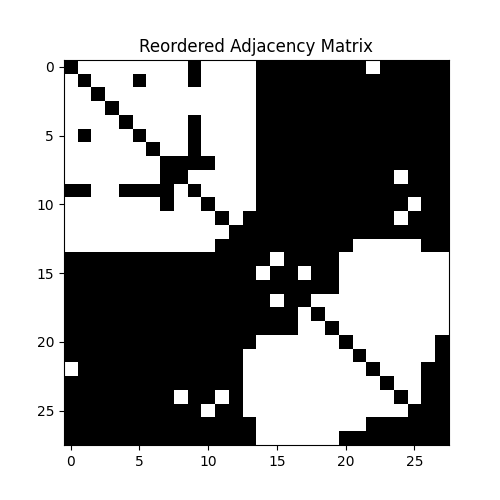
\includegraphics[width=0.7\linewidth]{figures/graph_02_adjacency_matrix.png}
    \end{minipage}\hfill
    \begin{minipage}{.45\textwidth}
      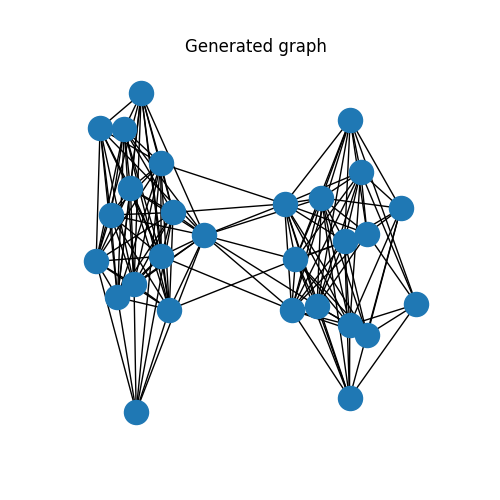
\includegraphics[width=0.7\linewidth]{figures/graph_02_generated_graph.png}
    \end{minipage}
  
    % Graph 03
    \begin{minipage}{.45\textwidth}
      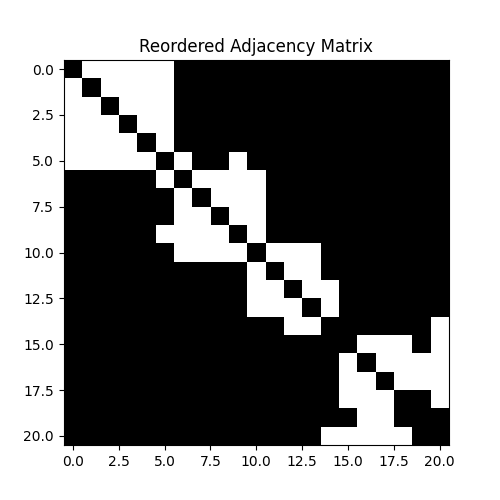
\includegraphics[width=0.7\linewidth]{figures/graph_03_adjacency_matrix.png}
    \end{minipage}\hfill
    \begin{minipage}{.45\textwidth}
      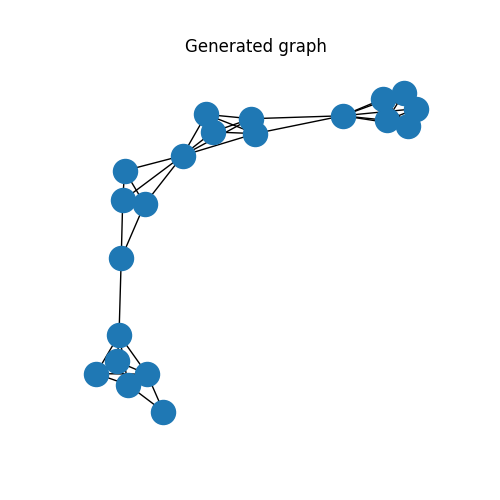
\includegraphics[width=0.7\linewidth]{figures/graph_03_generated_graph.png}
    \end{minipage}
  
    % Graph 04
    \begin{minipage}{.45\textwidth}
      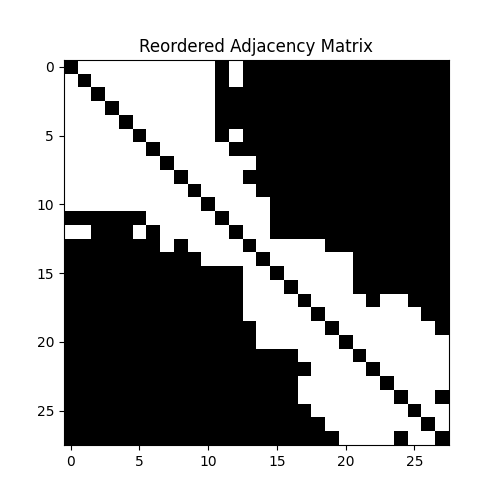
\includegraphics[width=0.7\linewidth]{figures/graph_04_adjacency_matrix.png}
    \end{minipage}\hfill
    \begin{minipage}{.45\textwidth}
      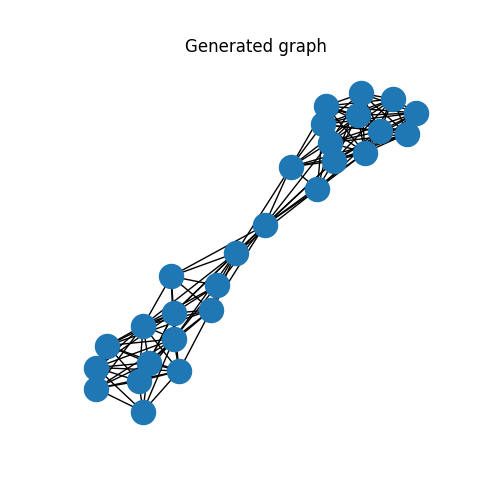
\includegraphics[width=0.7\linewidth]{figures/graph_04_generated_graph.png}
    \end{minipage}

\end{figure}

\end{document}